The tracking layer will consist of three subsystems and an interface. These subsystems are the tracking mode, tracking process, and GPI (Gaze Position Indicator).

\begin{figure}[h!]
	\centering
	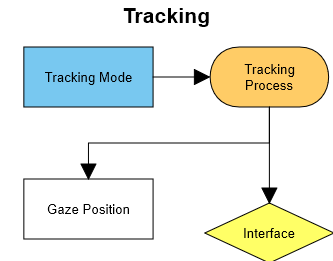
\includegraphics[width=0.60\textwidth]{images/tracking}
	\caption{Example subsystem description diagram}
\end{figure}

\subsection{Tracking Mode}
The tracking mode primarily consist of two states. Either controlling the cursor, or simply returning a set of screen coordinates that indicate the gaze position on the screen.

\subsubsection{Assumptions}
Project Iris has assumed that windows is the operating system being used, and that it's mousing API will not change significantly.

\subsubsection{Responsibilities}
It is this layers responsibility to determine if a set of coordinates are made available for API calls, or if the tracking algorithm is actively updating the systems mouse position.

\subsubsection{Subsystem Interfaces}

\begin {table}[H]
\caption {Subsystem interfaces} 
\begin{center}
    \begin{tabular}{ | p{1cm} | p{6cm} | p{3cm} | p{3cm} |}
    \hline
    ID & Description & Inputs & Outputs \\ \hline
    \#1 & Tracking Mode/Tracking Process & \pbox{3cm}{ } & \pbox{3cm}{Mode}  \\ \hline
    \end{tabular}
\end{center}
\end{table}

\subsection{Tracking Process}
The tracking process is the most important subsystem in all of Project Iris. It is where the gaze tracking algorithm will reside and also system updating will occur. The tracking process will calculate the position on screen based on gathered eye point data.  It will then use a smoothing algorithm to filter noise by using a quadratic technique to remove jitter.  Once after smoothed, if any point is calculated outside of the client window, the boundaries of the point are then recaculated to adjust to screen size.  If any point is greater than 30 degree angle of gaze then those gaze points will not be caculated and it will use the previous frame's position.

\subsubsection{Responsibilities}
It is this layers responsibility to actively track the users gaze position using data from the device layer and mode information from the mode layer.

\subsubsection{Subsystem Interfaces}

\begin {table}[H]
\caption {Subsystem interfaces} 
\begin{center}
	\begin{tabular}{ | p{1cm} | p{6cm} | p{3cm} | p{3cm} |}
		\hline
		ID & Description & Inputs & Outputs \\ \hline
		\#1 & Tracking Process/Tracking Mode & \pbox{3cm}{Mode} & \pbox{3cm}{ }  \\ \hline
		\#2 & Tracking Process/Interface & \pbox{3cm}{Raw Data\\Settings Changes} & \pbox{3cm}{Status}  \\ \hline
	\end{tabular}
\end{center}\textsl{}
\end{table}

\subsection{GPI (Gaze Position Indicator)}
The GPI subsystem will take the position provided by the tracking process and display a green graphical dot on the screen that indicates position.

\subsubsection{Subsystem Interfaces}

\begin {table}[H]
\caption {Subsystem interfaces} 
\begin{center}
	\begin{tabular}{ | p{1cm} | p{6cm} | p{3cm} | p{3cm} |}
		\hline
		ID & Description & Inputs & Outputs \\ \hline
		\#1 & Tracking Process/GPI & \pbox{3cm}{Gaze position} & \pbox{3cm}{ }  \\ \hline
	\end{tabular}
\end{center}
\end{table}

